%    Latex Template for ACA 2015
%%%%%%%%%%%%%%%%%%%%%%%%%%%%%%%%%%%%%%%%
%    DO NOT CHANGE THE SETTINGS BELOW
%%%%%%%%%%%%%%%%%%%%%%%%%%%%%%%%%%%%%%%%
\documentclass[11pt]{article}
\usepackage{epsfig}
\usepackage{graphicx}
\usepackage[latin1]{inputenc}
\usepackage[T1]{fontenc}
\usepackage{mathptmx}
\usepackage{url}

\begin{document}

%%%%%%%%%%%%%%%%%%%%%%%%
%%%%%%%%%%%%%%%%%%%%%%%%%%%%%%%%%%%%%%%%
%    DO NOT CHANGE THE SETTINGS ABOVE
%%%%%%%%%%%%%%%%%%%%%%%%%%%%%%%%%%%%%%%%
%
\vspace{-0.8cm}
\begin{flushleft}
\Large \textbf{\noindent
%%% PLEASE INSERT THE TITLE OF YOUR TALK HERE %%%%%%%
Improving mathematical competences by using modern technology}
%%%%%%%%%%%%%%%%%%%%%%%%%%%%%%%%%%%%%%%%%%%%%%%%%%%%%%%%
\\
%%%%%%%%%%%%%%%%%%%%%%%%%%%%%%
\vspace{0.5cm}
\normalsize
 %%%%%%             NAMES OF AUTHORS         %%%%%%
 %%%%%% NAME OF SPEAKER SHOULD BE UNDERLINED %%%%%%%%%
\normalsize{
 %%%%%% FOR EXAMPLE %%%%%
\underline{Jens Weitendorf}$^1$
 %%%%%%%%%%%%%%%%%%%%%%%%
} \\
\vspace{5mm}
\textit{\footnotesize
 %%%%%% AFFILIATION OF AUTHORS %%%%%%
$^1$ Norderstedt, Germany
JWeitendorf@t-online.de\\
 %%%%%%%%%%%%%%%%%%%%%%%%%%%%%%%%%%%%%
}
\end{flushleft}

Normally when you want to use modern technology in the classroom, you
are looking for exercises for those it is easier to solve them using
the technology.

In my talk I want to discuss an opportunity to deal with the curriculum on
a higher level. This means that you do not have to change the curriculum
but you have to change the point of view. The main issue will be the
functional aspect of mathematical ideas. For example if you discuss
the square function you can start with the universal form of the square
function and then the students will be able to find out the influence of
the three variables by themselves. Functions are represented by equations,
tables or graphs. Using technology it is quite easy to change between
those representations.

It will not be possible to discuss the whole curriculum. Therefore
I will put my focus on the curriculum for year 7 up to year 9/10 and
will give an idea, what is possible using technology. The way through
the curriculum will start with the percentage calculation and end with
exponential and trigonometric functions.  The helpful modern technology
will be the ClassPad 400.

To give an impression I will describe some examples. First I want to show
how linear equations can be solved by using the ClassPad or any other CAS.

\begin{figure}
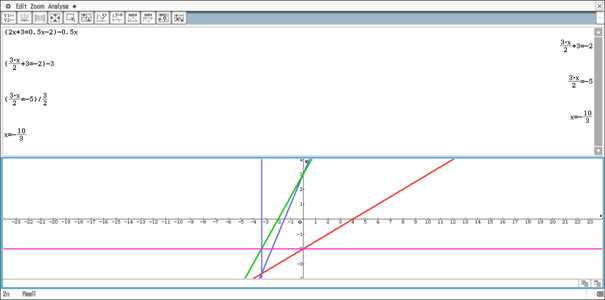
\includegraphics[width=\textwidth]{figure1.png}
\caption{Solving linear equations}
\label{Fig. 1}
\end{figure}

We start with the equation $2x + 3 = 0, 5x - 2$ (see fig. 1). You put
the equation in brackets and put the conversion behind. For students it
is helpful to do this because they only have to think about the way of
conversation and the calculator will do the calculation. Each part of the
equation is the term of a linear function. Therefore you can easily show
the corresponding graph. The solution of the equation is the x-value of
the point of intersection. The y-value changes. So it is necessary to
discuss the connections between changes in algebra and geometry.
The following mistake is quite popular:

\begin{eqnarray*}
3x + 4 & = & 7 | -3 \\
 x + 4 & = & 4
\end{eqnarray*}

The CAS will show the student that his idea will lead to: $3x + 1 =
4$. So the CAS will help to prevent those kinds of mistakes.

The next example will show the connection between a constructed curve
and the square function.

\begin{figure}
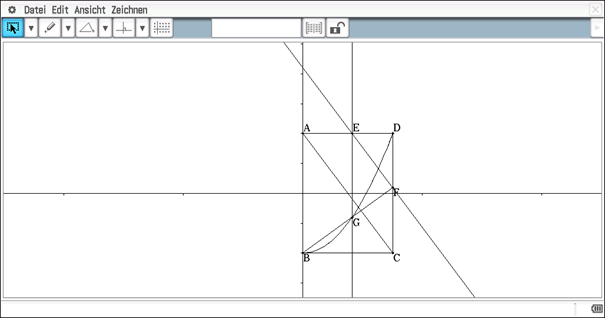
\includegraphics[width=\textwidth]{figure2.png}
\caption{Constructing a parabolic curve}
\label{Fig. 2}
\end{figure}

The rectangle ABCD is constructed (see fig. 2). The point E is put on
the line AD and a parallel to the diagonal AC is drawn. F is the point
of intersection and is connected with the point B of the rectangle. The
point G is the point of intersection between the line BF and the parallel
to the line DC through E. You will get the parabolic curve by animation
of the point E. The question is whether it is true that you have got
really a parabolic curve. The different coordinates of the point G are
saved by the ClassPad. Therefore it is possible to work with them in
the spreadsheet (see fig. 3).

\begin{figure}
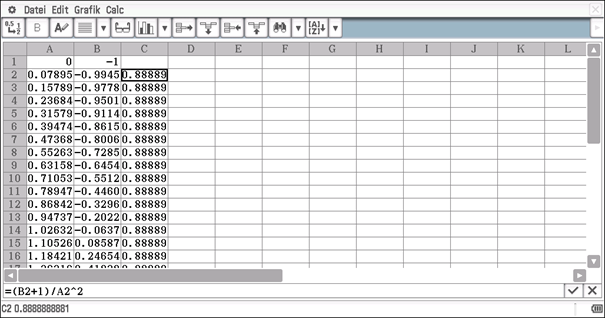
\includegraphics[width=\textwidth]{figure3.png}
\caption{Analysing the data}
\label{Fig. 3}
\end{figure}

This is not a proof of course, but it gives the students an idea
of working with data. The proof has to be done afterwards in the
classroom. And the question whether a proof is necessary or not must be
put up for discussion.

The last example will deal with a problem for older students.  We want
to get a formula for the curvature of a graph of a function. Therefore
you can start with a special function and a special point.

\begin{figure}
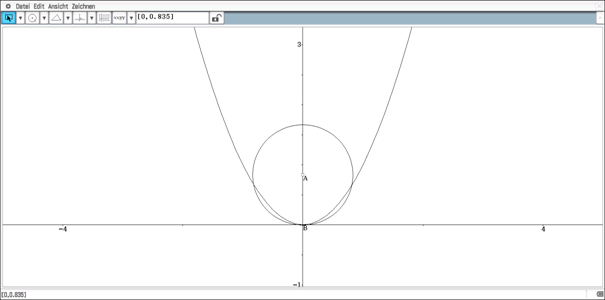
\includegraphics[width=\textwidth]{figure4.png}
\caption{Parabolic curve and responding circle}
\label{Fig. 4}
\end{figure}

We discuss the graph of the square function $f(x) = x^2$ and the point
$(0/0)$. A circle is constructed with centre $A$, which is variable on
the $y$-axis, and the point $B(0/0)$. The students can find out that the
circle and the parabolic curve have one or three common points. The
crossing-point is of special interest. This leads to the definition of
what is meant by the curvature of a graph.

In the situation of the crossing-point the following equations must
be true:
\begin{tabular}{ll}
Square function:    & $f(x) = x^2$ \\
Part of the circle: & $c(x)=r-\sqrt{r^2- x^2}$
\end{tabular}

The three equations:
$$
f(0) = c(0) \qquad f'(0) = c'(0) \qquad f''(0) = c''(0)
$$
You can generalize those three equations to any function and any point
and a CAS like the ClassPad will be able to create the formula.

%%%%%%%%%%%%%%%%%%%%%%%%%%%%%%%%%%%%%%%


%%%%%%%%%%%%%%%%%%%%%%%%%%%%%%%%%%%%%%%%
%% BIBLIOGRAPHY
%%%%%%%%%%%%%%%%%%%%%%%%%%%%%%%%%%%%%%%%
%\begin{thebibliography}{00}
%\addcontentsline{toc}{chapter}{References}
%\setlength{\itemsep}{-1mm}
%\footnotesize
%\bibitem{KR} B. Keller and I. Reiten, \textit{Cluster-titled algebras are Gorenstein and stably Calabi-Yau}, Adv. Math. \textbf{211}, 1, pp. 123-151 (2007).
%\bibitem{WK} S. Washito and K. Karabashi, \textit{Use This Template}, in \textit{Proceedings of the 5th
%International Conference on Photon Interaction} (ICPI-2012), San Francisco, USA, ed. A. Chen, pp. 22-24 (2012).
%\bibitem{ABS} A.B. Smith, \textit{Describing the style for the AMMCS-CAIMS-2015 book of abstracts}, in C.D. Science (ed.), General Book of Wisdom, 2\textsuperscript{nd} ed., University of Queensland, pp. 23-42 (2011).
%\end{thebibliography}
%\normalsize
\end{document} 
